\section{Introduction}
Despite the advent of more precise methods, the use of leaves to identify trees and other plants persists. The variance of shapes between species with a general uniformity of shape within one species, combined with the portability and size of the leaves, has ensured their popularity for this usage. 
Whereas leaf identification used to require manual comparison of the leaf (or a photograph of it) to images of previous leaves (often involving large decision trees), advances in computer vision have made fast, large scale comparison of images feasible \cite{Belh2008}. One example of the use of computer image classification for leafs is the LeafSnap app \cite{Kuma2012}: a mobile app covering all 185 species of the northeast USA, it enables users to photograph leaves and immediately classify them, by transmitting the captures image to a server which houses the recognition system. After classification, the user is presented with a sorted list of identification results from which they can pick the one that most resembles their leaf. Total time to solution after uploading of the image is 5.4 seconds \cite{Kuma2012}.

We decided to develop a system with a similar goal, to identify the species of a leaf by using Machine Learning techniques to compare it with a processed database of labelled examples. The resulting system is capable of performing the whole process: feature extraction from an image database and using the extracted features to train a classifier. We used a publicly accessible data set that was used in the ImageClef 2012 leaf classification challenge, earlier instalments of which have been used before in comparable efforts to make an image classification system \cite{Goea2011}. These systems usually innovate most in the mechanism chosen for feature extraction; classification of the extracted features is often achieved using established methods. For example, earlier work \cite{Kaly2015} used a combination of geometric features such as contour information and moment invariants, among others, and a linear discriminant classifier.
We decided to limit ourselves to one feature extraction method: a combination of Scale Invariant Feature Transform (SIFT) descriptors and Bag of Visual Words~\cite{Zhan2010}, and focus our efforts on the classification phase by using a custom Neural Network and comparing it to a simple K-Nearest Neighbour classifier.
We expected the neural network to come out on top in this comparison.
An overview of the method is provided  in Figure \vref{fig:overview}.

\begin{figure}[htb]
    \centering
    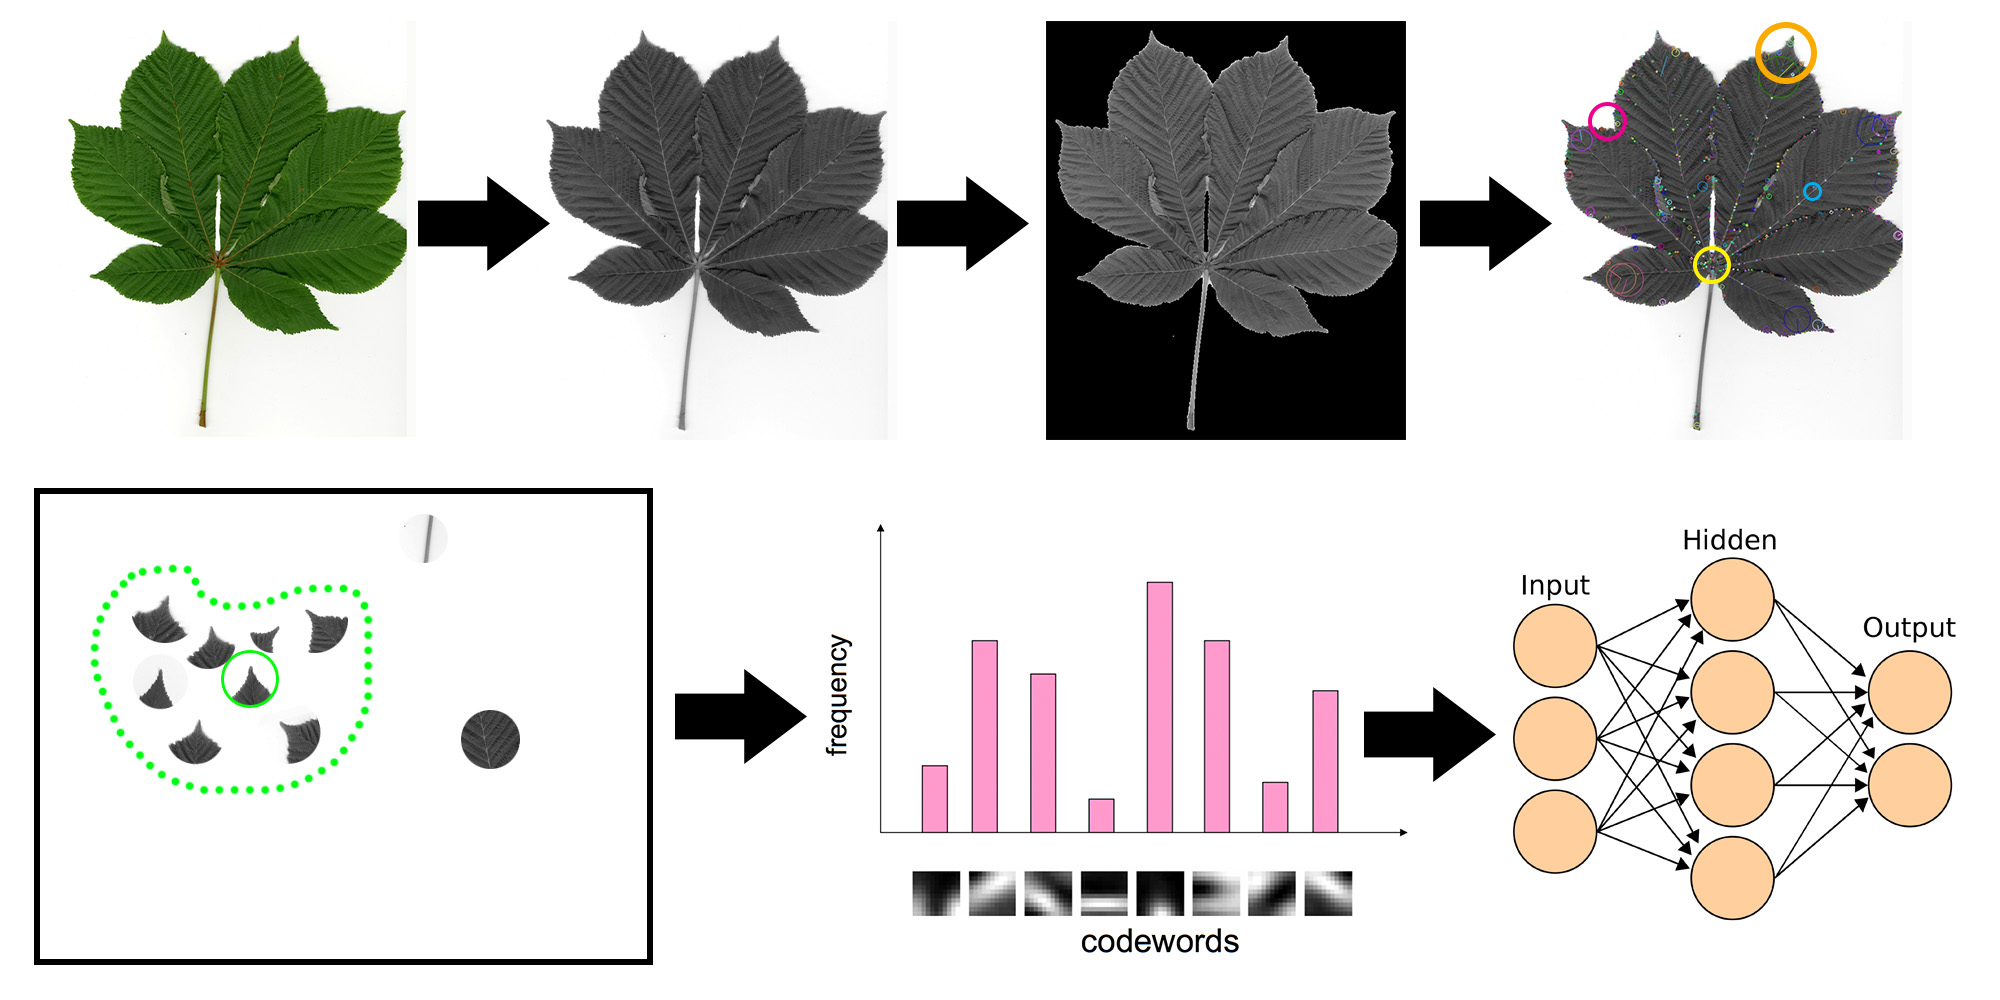
\includegraphics[width=0.8\textwidth]{flowchart.jpg}
    \caption{The classification procedure}
    \label{fig:overview}
\end{figure}


Our expectations were modest, emphasizing the development of a working system that would run on a normal PC, and be capable of classifying leaf images at a rate substantially higher than that of a random guess. Other, more advanced, programs have been shown to be in the 90\% accuracy range \cite{Wang2011, Kaly2015}.
However, the simpler approach taken in this study may have its benefits too. Speed of classification is of paramount importance, especially when the classifier is used in a real-world context, such as in a smartphone app. Users may be more than willing to trade in some accuracy if it means that they get an answer more quickly. The computational limitations of small devices such as smartphones may also tip the balance towards a classifier that uses its resources sparingly. 
The methods used in this study may be seen as an attempt to address these concerns, by exploring the effect on performance of a stronger emphasis on simplicity.

Finally, it is important to note that accuracies are not easily compared across the various systems mentioned here, as leaf classification systems such as LeafSnap tend to present a top 5 of solutions; in some cases, having the correct class appear in the top N list is counted as a successful classification \cite{Wang2011}.
 	